\documentclass[10pt]{article}
\usepackage{amsmath}
\usepackage{graphicx}
\usepackage{float}
\usepackage{subfig}
\usepackage{epsfig}
\usepackage{color}
%---------------------------------------------------------------------------
%
%          USER DEFINED MACROS
%
%\mathsurround = 2pt


\def \ds          {\displaystyle}
\def \rmd         {{\rm d}}
\def \be          {{\bf e}}
\def \bF          {{\bf F}}
\def \bI          {{\bf I}}
\def \bn          {{\bf n}}
\def \bff         {{\bf f}}
\def \bdf         {{\bf df}}
\def \bdT         {{\bf dT}}
\def \bT          {{\bf T}}
\def \cT          {{\cal T}}
\def \bU          {{\bf U}}
\def \bu          {{\bf u}}
\def \bv          {{\bf v}}
\def \bV          {{\bf V}}
\def \bX          {{\bf X}}
\def \by          {{\bf y}}
\def \bY          {{\bf Y}}
\def \bz          {{\bf z}}
\def \bZ          {{\bf Z}}
\def \bW          {{\bf W}}
\def \bZt         {{\bf \widetilde Z}}
\def \bzi         {{\bz}_i}
\def \bzs         {{\bz}^*}
\def \bzis        {{\bz}_i^*}
\def \bzin        {\{\bzi\}_{i=1}^k}
\def \cf          {{\cal F}}
\def \cg          {{\cal G}}
\def \ch          {{\cal H}}
\def \vi          {{V_i}}
\def \vin         {\{\vi\}_{i=1}^k}
\def \Babs        {{\Big|}}
\def \Bl          {{\Big(}}
\def \Br          {{\Big)}}
\def \Bleft       {{\Big[}}
\def \Bright      {{\Big]}}
\def \p           {\partial}
\def \R           {{\mathbb R}}
\def \N           {{\mathbb N}}
\def\y            {{\bf y}}
\def \tN          {{\widetilde{N}}}
\def \tD          {{\widetilde{D}}}

\def\m*         #1{m^{*}(\,#1\,)}
\def \proofnote #1{\footnote{{\bf Note: #1}}}
\def \norm      #1{\left|\,#1\,\right|}
\def \set       #1{\left\{\,#1\,\right\}}
\def \tr          {^T}
\def \IhH         {I_h^H}
\def \IhHb        {{\hat I}_h^H}
\def \IHh         {I_H^h}
\def \vbar        {\bar \bv}
\def \zhbar       {\bar \bz_h}
\def \zHbar       {\bar \bz_H}
\def \zhplus      {\bz_h^+}
\def \zHplus      {\bz_H^+}

\renewcommand{\theequation}{\thesection.\arabic{equation}}

\newtheorem{alg}{Algorithm}[section]
\newtheorem{thm}{Theorem}[section]
\newtheorem{lem}[thm]{Lemma}
\newtheorem{cor}[thm]{Corollary}
\newtheorem{pro}{Proposition}[section]
\newtheorem{defn}{Definition}[section]
\newtheorem{asp}{Assumption}[section]
\newtheorem{rmk}{Remark}[section]

%\def \Rblack#1{\,\hbox{R \kern-1.2em I
%    \kern.275em $^{#1}$}}
%\def \bG{{\bf G}}
%\def \bt{{\bf t}}
%\def \bzj{{\bz}_j}
%\def \bY{{\bf Y}}
%\def \byi{{\by}_i}
%\def \byj{{\by}_j}
%\def \byim{\{\byi\}_{i=1}^m}
%\def \bx{{\bf x}} 
\title{\ Progress Report until May 26}
\author{Zichao Di}
\date{\today}
\begin{document}
  \maketitle 

\section {Issues about active set method in TN}
\begin{itemize}
\item Some coding issues in 'lmqnbcm' \footnote{\bf Note:the same issues happen in 'lmqnbc' as well} may result in the maximum step length $\alpha_{0}=0$ for the line search
\begin{itemize}
\item In 'lmqnbcm', the process is to update the active set first and then to calculate the maximum step length considering every variable in the active set. According to this, it may take the binding variable into consideration to calculate the maximum step length which may result into $\alpha_{0}=0$
\end{itemize}
\item What I modified  is to apply one more 'modz' before calculating $\alpha_{0}$ which as follows:
\begin{quote}
\begin{verbatim}
 if (abs(alpha-spe) <= 10*eps);
        ipivot0 = ipivot;
        newcon = 1;
        [ipivot, flast] = modz (x, p, ipivot, low, up, flast, f, alpha);
 end;
 spe = stpmax (stepmx, pe, x, p, ipivot, low, up);
 alpha = step1 (f, gtp, spe);
 alpha0 = alpha;
\end{verbatim}
\end{quote}
In this way, it will exclude any current binding variable into account.
\item In figure \ref{fig:2side}, it shows the improvement of MG/OPT on 2-side bound problem\footnote{\bf: Note: All the following tests are based on the original setting of line search in both TN and mgrid}.
\end {itemize}
\begin{figure}[h]
\centering
  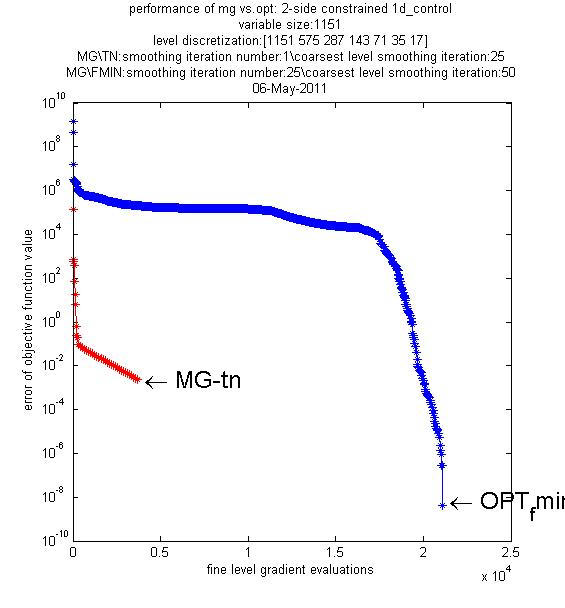
\includegraphics[width=1.0\textwidth]{2-side-evalgrad.jpg}
  \caption{2-side bounds problem:  Improved fine level gradient evaluation according to the modification in 'lmqnbcm'}
\label{fig:2side}
\end{figure}

\section{Some Analysis in 1-side bound problem}
\begin{itemize}
\item My next task is to try to fix the issue happend in the error between downdate of variable and the original fine level which will force the fine-level variable out of bound after being updated by the coarse solution
\item Firstly, I did some analysis on the original problem to find a proper corresponding coarse problem constraint.
\begin{itemize}
\item The original quadratic problem : $f(x)=1/2x^{T} Ax-b^{T} x$ s.t.$x\geq l$
\item Our goal is to minimize 
$$f(v_{h}+\IHh(e_{2}-v_{H}))$$
$$=1/2(v_{h}+\IHh(e_{2}-v_{H}))^{T}A_{h}(v_{h}+\IHh(e_{2}-v_{H}))-b_{h}^{T}(v_{h}+\IHh(e_{2}-v_{H}))$$	
$$=1/2v_{h}^{T}A_{h}v_{h}+1/2(\IHh(e_{2}-v_{H}))^{T}A_{h}v_{h}+1/2v_{h}^{T}A_{h}(\IHh(e_{2}$$
%$$\quad \quad -v_{H}))+1/2(\IHh(e_{2}-v_{H}))^{T}A_{h}(\IHh(e_{2}-v_{H}))-b_{h}^{T}v_{h}-b_{h}^{T}(\IHh(e_{2}-v_{H}))$$

%$$=f(v_{h})+(\IHh(e_{2}-v_{H}))^{T}A_{h}v_{h}+1/2(\IHh(e_{2}-v_{H}))^{T}A_{h}(\IHh(e_{2}-v_{H}))-b_{h}^{T}(\IHh(e_{2}-v_{H}))$$

$$=f(v_{h})+\tilde{f}(e_{2})$$ where $\tilde{f}(e_{2})=1/2(\IHh(e_{2}-v_{H}))^{T}A_{h}(\IHh(e_{2}-v_{H}))+\tilde{b}^{T}(\IHh(e_{2}-v_{H}))$ in which $\tilde{b}=A_{h}v_{h}-b_{h}$\\

Since we have $\IHh=2 (\IhH)^{T}\implies (\IHh)^{T}=2\IhH$. And also we know that in MG/OPT, the shifted coarse function is defined as $$f_{H}^{s}=f_{H}(x)-(\nabla f_{H}(v_{H})-\IhH \nabla f_{h}(v_{h}))^{T}x$$
$$=1/2x^{T}A_{H}x-b_{H}^{T}x+(\IhH A_{h}v_{h}-A_{H}v_{H})^{T}x$$
$$\tilde{f}(e_{2})=(v_{h}^{T}-b_{h}^{T})(\IHh e_{2})-(v_{h}^{T}A_{h}-b_{h}^{T})\IHh v_{H}+1/2((\IHh e_{2})^{T}A_{h}(\IHh e_{2}))$$
$$\quad \quad -((\IHh V_{H})^{T}A_{h}(\IHh e_{2}))+1/2((\IHh v_{H})^{T}A_{h}(\IHh v_{H}))$$
$$=v_{h}^{T}A_{h}\IHh e_{2}-b_{h}^{T}\IHh e_{2}+\frac{1}{2} 2 e_{2}^{T}A_{H}e_{2}-\frac{1}{2} 2 e_{2}^{T}A_{H}v_{H}-\frac{1}{2} 2 v_{H}^{T}A_{H}e_{2}+C$$ 
$$=2f_{H}^{s}(e_{2})+C$$ where $C=-(v_{h}^{T}A_{h})\IHh v_{H}+b_{h}^{T}\IHh v_{H}+\frac{1}{2} 2 v_{H}^{T}A_{H}v_{H}$\\

On coarse level, we have $e_{2,0}=v_{H}$. Thus $$f(v_{h}+\IHh(e_{2}-v_{H}))=f(v_{h})+\tilde{f}(e_{2})\leq f(v_{h})+\tilde{f}(v_{H})=f(v_{h})$$

Therefore, $min\, f(v_{h}+\IHh(e_{2}-v_{H}))$ is equivalent to $min\, \tilde{f}(e_{2})$, then it turns out to be equivalent to minimize $f_{H}^{s}(e_2)$. Also, in order to force $v_{h}+\IHh(e_{2}-v_{H})\geq l$, let the lower bound of coarse problem is $l_{H}$, then $$l_{H,i}=max(l_{2i}\, ,\, l_{2i}+1/4v_{h,2i-1}-1/2 v_{h,2i}+1/4 v_{h,2i+1})$$\\

Proof:For even nods:
$$v_{h,2i}+\IHh(e_{2,i}-v_{H,i})$$
$$\geq v_{h,2i}+\IHh(l_{2i}+1/4v_{h,2i-1}-1/2 v_{h,2i}+1/4 v_{h,2i+1}-v_{H,i})$$
$$= v_{h,2i}+l_{2i}+1/4v_{h,2i-1}-1/2 v_{h,2i}+1/4 v_{h,2i+1}-(1/4v_{h,2i-1}+1/2 v_{h,2i}+1/4 v_{h,2i+1})$$
$$=l_{2i}$$ 
For odd nods: 
$$v_{h,2i-1}+1/2(e_{2,i-1}-v_{H,i-1})+1/2(e_{2,i}-v_{H,i})$$
$$=v_{h,2i-1}+1/2(e_{2,i-1}+e_{2,i})-1/2(1/2v_{h,2i-3}+1/2v_{h,2i-2}+1/2v_{h,2i-1}+1/2v_{h,2i}+1/4v_{h,2i+1})$$
$$\geq (3/4-1/8-2/8-2/8-1/8)l_{h,2i-1}+1/2(l_{H,i-1}+l_{H,i})$$. Thus, choose $l_{H}=l_{h}$ will satisfy the bound constraint.


\end{itemize}

\item According to following analysis, I found a mistake in the setting up of all parameters, before, I calculate $b$ separately in different levels following the same fomular, acutally, $b_{H}=\IhH b_{h}$.

\item Then apply all above conclusions to the code, I get the figure \ref{fig:newb} from which, we can see that MG/OPT can get to at least the same accuracy as OPT along with its benefit.
\begin{figure}[h]
\centering
  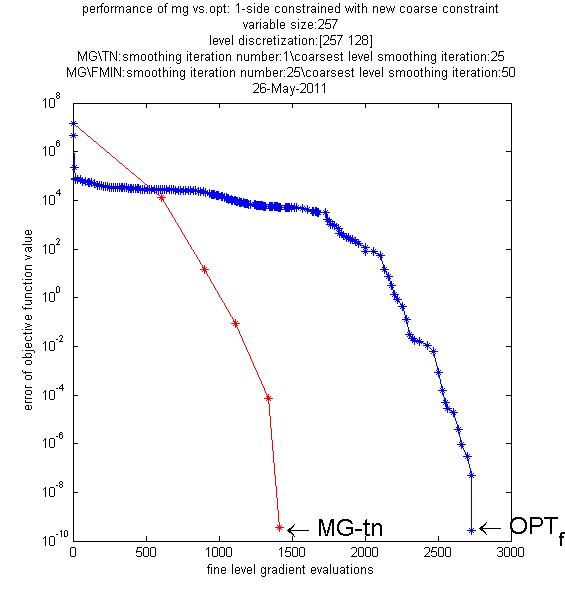
\includegraphics[width=1.0\textwidth]{newcoarsebound257.jpg}
  \caption{1-side bounds problem:  Improved fine level gradient evaluation according to the modified coarse constraint}
\label{fig:newb}
\end{figure}



\item I also tried the constraint in Toint, since its setting of $l_{H,i}=v_{H,i}+max(l_{h}-v_{h})$, since along with the showing of binding variable, the second component of above equation will be zero, so the coarse problem will only supply very tiny step since no more room for the $v_{H}$ to move, so it fails.
\end{itemize}

\section {Next step:}
\begin{itemize}
\item Try to implement the code for more than 2 levels, the comlication is I have to fix the constraint in each coarse level corresponding to its right fine level.
\end{itemize}


























\end{document}
